\documentclass[letterpaper,12pt]{scrartcl}
\usepackage{epsfig,latexsym,amsmath,amssymb,epic,eepic,psfrag,subfigure,float,euscript,array}
\usepackage[latin1]{inputenc}
\usepackage[margin=24mm]{geometry}
\usepackage{tikz,pgf,pgfplots}
\usepgfplotslibrary{fillbetween}
\usepgfplotslibrary{groupplots}
\usetikzlibrary{decorations, arrows, fit, circuits.plc.ladder}

\usepackage[amssymb]{SIunits}

\newenvironment{exercise}[1][Exercise]{\begin{trivlist} \item[\hskip
    \labelsep {\stepcounter{exerctr}\bfseries #1
      \arabic{exerctr}}]}{\end{trivlist}\vspace{10mm}}

\newcounter{exerctr}
\newcounter{abcctr}[exerctr]

\newcommand{\abc}{\noindent\vspace{1mm}\\ \textbf{
    \stepcounter{abcctr}(\alph{abcctr})\ }}
\newcommand{\bbm}{\begin{bmatrix}}
\newcommand{\ebm}{\end{bmatrix}}
\newcommand{\point}[1]{\hfill \textbf{ (#1p)}\\ \vspace{-5mm}}
\newcommand{\ctrb}{\EuScript{S}}
\newcommand{\Lap}{\mathcal{L}}
\newcommand{\obsv}{\EuScript{O}}
\newcommand{\realdel}{\text{Re}}
\newcommand{\imagdel}{\text{Im}}
\newcommand{\bC}{\mathbb{C}}
\newcommand{\bR}{\mathbb{R}}
\newcommand{\bmpv}{\begin{minipage}[t]}
\newcommand{\bmps}{\begin{minipage}[t]{45mm}}
\newcommand{\bmpm}{\begin{minipage}[t]{90mm}}
\newcommand{\bmpl}{\begin{minipage}[t]{\textwidth}}
\newcommand{\emp}{\end{minipage}}
\newcommand{\mexp}[1]{\ensuremath{\mathrm{e}^{#1}}}

\newcommand{\AxisRotator}[1][rotate=0]{%
    \tikz [x=0.2cm,y=0.60cm,line width=.1ex,-stealth,#1] \draw (0,0) arc (-150:150:1 and 1);%
}

%\addtolength{\topmargin}{-1cm}
%\textheight 22.5cm
%\oddsidemargin 1.3cm
%\evensidemargin 1.3cm

\makeatletter
\newcommand*{\rom}[1]{\expandafter\@slowromancap\romannumeral #1@}
\makeatother

\newcommand*\circled[1]{\tikz[baseline=(char.base)]{
            \node[shape=circle,draw,inner sep=2pt] (char) {#1};}}


\title{Modeling and automation - Exam group 301}
\author{Kjartan Halvorsen}
\date{2022-06-09}

\begin{document}

\maketitle


\begin{description}
\item[Time] 17:05 - 18:55
\item[Permitted aids] The single page with your own notes, table of Laplace transforms, calculator
\end{description}

All answers should be readable and well motivated (if nothing else is written). Solutions/motivations should be written on the provided spaces in this exam. Use the last page if more space is needed.

\begin{center}
{\Large Good luck!} \\
\end{center}

\noindent
\fbox{
\bmpl
\textbf{ Matricula and name:}\\
\vspace*{14mm}
\emp}


%\clearpage

%-----------------------------------------------------------------

\section*{Magnetic levitation}
\label{sec-1}

Figure \ref{fig:magnetic-suspension} shows a one-dimensional magnetic suspension system. The current $i$ in the windings generates a magnetic field which suspends the mass $m$. Friction is completely negligable, since the mass is not in contact with any other body, and its velocity is typically very small (no air-drag). Hence, there are two forces acting on the mass: gravity and the magnetic force. The magnetic force is proportional to the square of the current $i$ and inverse proportional to the square of the gap distance $x$. This gives the equation of motion 
\begin{equation}
m \ddot{x} = -C \left( \frac{i}{x} \right)^2 + mg.
\label{eq:magode}
\end{equation}
Introduce the variable
\[ z(t) = \big(i(t)\big)^2,\]
with which the ODE can be written
\begin{equation}
\ddot{x} = -\frac{Cz}{mx^2} + g.
\label{eq:magodenew}
\end{equation}

\begin{figure}[htb]
\begin{center}
\includegraphics[width=0.5\linewidth]{../figures/magnetic-suspension}
\caption{A magnetic suspension system. The force of gravity acts to pull the mass $m$ downwards. The force due to the magnetic field generated by the current $i$ keeps the mass from falling down. The displacement $x$ of the mass is positive downwards.}
\label{fig:magnetic-suspension} 
\end{center}
\end{figure}
The system is non-linear, so in order to use linear control design, the system must be linearized about an operating point. Introduce the deviation variables \(y\) and \(u\)
\begin{align*}
x(t) &= x_0 + y(t) \\
z(t) &= z_0 - u(t).
\end{align*}
The input signal to the system is the change, $u$, in the square of the current in the windings, and the output signal is the change, \(y\),  in the gap distance. 
\begin{center}
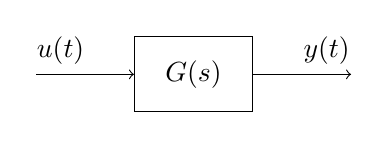
\begin{tikzpicture}[node distance=20mm,
                    block/.style={rectangle, draw, minimum width=15mm, inner sep=3mm},
                    sumnode/.style={circle, draw, inner sep=3pt}]
  \node[coordinate] (input) {};
   \node[block, right of=input,] (lti) {$G(s)$};
   \node[coordinate, right of=lti,] (output) {};
   \draw[->] (input) -- node[near start, above] {$u(t)$}  (lti);
   \draw[->] (lti) -- node[coordinate] (meas) {} node[near end, above] {$y(t)$} (output);
 \end{tikzpicture}
\end{center}
The negative sign in the definition of the deviation variable $u$,  \(z = z_0 - u\), is introduced so that a positive input signal leads to a positive change in the gap distance.

\begin{exercise}
\abc
Show that given an operating point $x_0$, the corresponding operating point $z_0$ that gives equilibrium is
\[ z_0 = x_0^2\frac{mg}{C}.\]

\noindent
\fbox{
\bmpl
\textbf{ Calculations:}\\
\vspace*{40mm}
\emp}



\abc
Show that the linearized model of the magnetic levitator system becomes
\begin{equation}
\ddot{y} = 2\frac{Cz_0}{mx_o^3}(x - x_0) - \frac{C}{mx_0^2}(z-z_0) = \frac{2g}{x_0} y + \frac{C}{mx_0^2} u
\label{eq:linearode}
\end{equation}

\noindent
\fbox{
\bmpl
\textbf{ Calculations:}\\
\vspace*{100mm}
\emp}

\abc
Determine the transfer function of the linear model \eqref{eq:linearode}.

\noindent
\fbox{
\bmpl
\textbf{ Calculations:}\\
\vspace*{60mm}
\emp}


\abc
[Bonus exercise worth 5p] Find the poles of the system and determine if the system is stable or not.

\noindent
\fbox{
\bmpl
\textbf{ Calculations:}\\
\vspace*{50mm}
\emp}
\end{exercise}



%\begin{equation}
%G(s) = \frac{ \frac{ 2\sqrt{Cg} }{\sqrt{m} x_0} }{s^2 - \frac{2g}{x_0}}.
%\end{equation}
%The system is unstable, with poles in \(\pm \sqrt{\frac{2g}{x_0}}\). Normalizing the time (using the unit of time \(T=\sqrt{\frac{x_0}{2g}}\)) and setting $u(t) = \frac{2\sqrt{Cg}}{\sqrt{m}x_0} \tilde{i}(t)$ gives the plant model
%\begin{equation}
%Y(s) = G(s)U(s) = \frac{1}{s^2 - 1} U(s).
%\label{eq:trf}
%\end{equation}



\section*{A Coupled spring-mass system}
The figure below shows a system consisting of two masses connected together and to two rigid walls.
\begin{center}
  \includegraphics[width=0.75\linewidth]{../figures/two-masses-spring-damper-2}
\end{center}
The displacements $z_1$ and $z_2$ are deviations from the equilibrium positions of the two masses, respectively, when the force $F(t)$ acting on the right mass is zero. The springs and dampers are considered to be linear. 

\subsection*{Problems}
\begin{exercise}
\abc
Draw free-body-diagrams and determine the differential equations that describe the system.

\noindent
\fbox{
\bmpl
\textbf{ Calculations:}\\
\vspace*{80mm}
\emp}

\abc
Choose a suitable state vector $x$, and write the system on state-space form
\begin{align*}
  \dot{x}(t) &= Ax(t) + B\,F(t)\\
  y(t) &= C x(t)
\end{align*}
where the output signal consists of the positions of the two masses, $y=\bbm z_1\\z_2\ebm$.

\noindent
\fbox{
\bmpl
\textbf{ Calculations:}\\
\vspace*{90mm}
\emp}

\end{exercise}



\cleardoublepage
% \end{document}

\section*{Solutions}
\setcounter{exerctr}{0} 

\subsection*{Magnetic levitation}
\begin{exercise}

  \abc
  At equilibrium the gravitational force and the magnetic force are equal in magnitude but opposite.
  \[ 0 = -C\frac{z_0}{mx_0^2} + g, \quad \text{Solve for $z_0$}\]
  \[ z_0 = x_0^2\frac{mg}{C}.\]

  \abc
  We write the nonlinear ODE as
  \[ \ddot{x} = -\frac{Cz}{mx^2} + g = f(z,x),\]
  and linearize the nonlinear right-hand side about the operating point $x_0$, $z_0$:
  \begin{align*}
    f(z,x) &\approx f(z_0, x_0) + \frac{\partial f}{\partial x}\Big|_{z_0, x_0} (x-x_0)
             + \frac{\partial f}{\partial z}\Big|_{z_0, x_0}(z-z_0)\\
           &= \underbrace{-\frac{Cz_0}{mx_0^2} + g}_{=0} + \frac{2Cz_0}{mx_0^3}\underbrace{(x-x_0)}_{y}
             - \frac{C}{mx_0^2}\underbrace{(z-z_0)}_{-u}\\
           &= \frac{2Cx_0^2mg}{Cmx_0^3} y + \frac{C}{m x_0^2} u\\
           &= \frac{2g}{x_0}y + \frac{C}{mx_0^2} u.
  \end{align*}
  The left-hand side of the ODE becomes
  \[ \ddot{x} = \ddot{x_0} + \ddot{y} = \ddot{y}. \]
  
  \abc
  Lumping the parameters (to make life easier), $a = \frac{2g}{x_0}$, $b = \frac{C}{mx_0^2}$,  
  taking the Laplace transform of each term in the model \eqref{eq:linearode}, and setting all initial values to zero (we are interested in the transfer function, not the transient response to the initial value) gives
  \[ s^2 Y(s) = aY(s) + bU(s),\]
which solved for $Y(s)$ is
\[ Y(s) = \frac{b}{s^2 - a} U(s).\]
Hence, the transfer function is  \[G(s) = \frac{cs}{s^2 - a}.\]

\abc
The poles are found by setting the denominator of the transfer function to zero, i.e.~formulating the characteristic equation
\[ s^2 + a = 0 \quad \Rightarrow \quad s = \pm \sqrt{a}.\]
The poles are real, and symmetric about the imaginary axis. The pole $s=\sqrt{a}$ is in the right-half plan, and so the system is unstable.
\end{exercise}


\subsection*{Spring-mass system}

\begin{exercise}
  \abc
  Free-body-diagrams of the two bodies give
  \begin{center}
    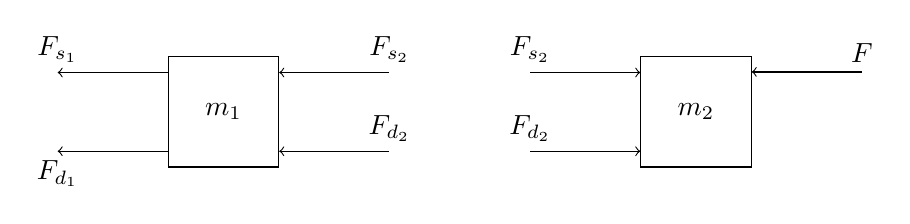
\begin{tikzpicture}
      \node[draw, minimum height=14mm, minimum width=14mm] (m1) {$m_1$};
      \draw[->] (m1.west) ++(0, 5mm) -- ++(-14mm, 0) node[above] {$F_{s_1}$};
      \draw[->] (m1.west) ++(0, -5mm) -- ++(-14mm, 0) node[below] {$F_{d_1}$};
      \draw[<-] (m1.east) ++ (0, 5mm)  -- ++(14mm, 0) node[above] {$F_{s_2}$};
      \draw[<-] (m1.east) ++ (0, -5mm)  -- ++(14mm, 0) node[above] {$F_{d_2}$};

      \begin{scope}[xshift = 6cm]
      \node[draw, minimum height=14mm, minimum width=14mm] (m2) {$m_2$};
      \draw[<-] (m2.west) ++ (0, 5mm) -- ++(-14mm, 0) node[above] {$F_{s_2}$};
      \draw[<-] (m2.west) ++ (0, -5mm) -- ++(-14mm, 0) node[above] {$F_{d_2}$};
      \draw[<-] (m2.north east) ++ (0,-2mm)  -- ++(14mm, 0) node[above] {$F$};
    \end{scope}
    \end{tikzpicture}
  \end{center}
  where the spring forces are given by
  \[ F_{s_1} = k_1z_1, \qquad F_{s_2} = k_2(z_1-z_2), \]
  and the damper forces
  \[ F_{d_1} = b \dot{z}_1, \qquad F_{d_2} = b(\dot{z}_1 - \dot{z}_2).\]
  Newton's second law for each body gives
  \begin{align*}
    m_1\ddot{z}_1 &= - F_{s_1} - F_{s_2} - F_{d_1} - F_{d_2} = - k_1z_1 - k_2(z_1-z_2) -b\dot{z}_1 - b(\dot{z}_1 - \dot{z}_2)\\
    m_2\ddot{z}_2 &=  -F + F_{s_2}  + F_{d_2} = -F + k_2(z_1-z_2) + b(\dot{z}_1 - \dot{z}_2).
  \end{align*}

  \abc
  One natural choice (among various) of the state vector is
  \[ x = \bbm x_1\\ x_2 \\x_3 \\x_4 \ebm = \bbm z_1\\ \dot{z}_1 \\z_1-z_2 \\\dot{z}_2 \ebm, \]
  where we focuse on the four energy-storing elements of the system (the deflection of the two springs, and the velocities of the two masses). with this choice, the differential equations can be written
  \begin{align*}
    \dot{x}_1 &= \dot{z}_1 = x_2\\
    \dot{x}_2 &= \ddot{z}_1 = -\frac{k_1}{m_1} z_1 - b\frac{b}{m_1}\dot{z}_1 - \frac{k_2}{m_1}(z_1-z_2) -\frac{b}{m_1}\dot{z}_1  + \frac{b}{m_1}\dot{z}_2 = -\frac{k_1}{m_1}x_1  - \frac{2b}{m_1}x_2  -\frac{k_2}{m_1}x_3  + \frac{b}{m_1}x_4\\
    \dot{x}_3 &= \dot{z}_1 - \dot{z}_2 = x_2 - x_ 4\\
    \dot{x}_4 &= \ddot{z}_2 = \frac{k}{m_2}(z_1 - z_2) + \frac{b}{m_2}\dot{z}_1 - \frac{b}{m_2}\dot{z}_2 - \frac{1}{m_2}F = \frac{b}{m_2}x_2 + \frac{k_2}{m_2}x_3 - \frac{b}{m_2}x_4 - \frac{1}{m_2}F. 
  \end{align*}
  The state-space model becomes
  \begin{align*}
    \dot{z} &= \bbm 0 & 1 & 0 & 0\\
    -\frac{k_1}{m_1} & -\frac{2b}{m_1} & -\frac{k_2}{m_1} & \frac{b}{m_1} \\
    0 & 1 & 0 & -1\\
    0 & \frac{b}{m_2} & \frac{k_2}{m_2} & -\frac{b}{m_2} \ebm x
                                        + \bbm 0\\0\\0\\-\frac{1}{M}\ebm F\\
    y &= \bbm z_1\\z_2\ebm = \bbm 1 & 0 & 0 & 0\\1 & 0 & -1 & 0\ebm x.
  \end{align*}
\end{exercise}
\end{document}


